
\documentclass{jtetiproposalskripsi}

%-----------------------------------------------------------------
%Disini awal masukan untuk data proposal tugas akhir
%-----------------------------------------------------------------
\titleind{PERANCANGAN SISTEM INFORMASI ABSENSI SISWA BERBASIS WEB MENGGUNAKAN SMS GATEWAY DI SMKN 5 JEMBER}
\fullname{NIDA KOMARIAH}

\idnum{1200631028}

\approvaldate{14 Januari 2015}

\degree{Diploma Manajemen Informatika}

\yearsubmit{2015}

\program{Manajemen Informatika}

\headprogram{Sarjiya, S.T., M.T., Ph.D.}

\dept{}

\firstsupervisor{Triawan Adi Cahyanto,M.Kom}
\firstnip{12 03 719}

\secondsupervisor{Bagus Setya Rintyarna,S.T,M.Kom}
\secondnip{09 03 521}


%-----------------------------------------------------------------
%Disini akhir masukan untuk data proposal skripsi
%-----------------------------------------------------------------

\begin{document}

\cover

\approvalpage

%-----------------------------------------------------------------
%Disini akhir masukan untuk muka skripsi
%-----------------------------------------------------------------

%-----------------------------------------------------------------
%Disini awal masukan Intisari
%-----------------------------------------------------------------
\begin{abstractind}
SMKN 5 JEMBER masih memiliki banyak kekurangan dalam pemenuhan akses pada sistem informasi sekolah, terutama untuk menangani sistem akademik, seperti kehadiran sistem informasi siswa, informasi jadwal, dan pengumuman penting dari sekolah. Sistem informasi yang masih manual yaitu, siswa dan orang tua harus datang ke sekolah untuk mendapatkan informasi tentang kehadirannya, atau masih menggunakan surat untuk menyampaikan informasi sekolah kepada orang tua siswa, dan sering menjadi kendala bagi orang tua yang sibuk dengan pekerjaan dan profesi mereka , atau putra dan putri yang kurang terbuka untuk orang tua.
Untuk mengatasi masalah itu terjadi, maka diperlukan sistem informasi yang dapat dilakukan dengan cepat, di mana pun, kapan saja, dan dalam hitungan detik pesan ke orang tua. Dengan membangun sistem informasi absensi siswa berdasarkan Short Message Service (SMS) Gateway yang merupakan pintu gerbang untuk memberikan informasi, dan dapat solusi untuk membantu siswa dan orang tua siswa dalam memperoleh informasi kehadiran, informasi jadwal, dan pengumuman penting dari sekolah.
Dengan menerapkan desain kehadiran sistem informasi siswa di SMKN 5 JEMBER berdasarkan SMS gateway diharapkan untuk membuatnya lebih mudah untuk mengelola informasi absensi siswa, informasi jadwal, dan pengumuman penting dari sekolah.

\begin{flushleft}
\textbf{Kata Kunci} : \textit{SMS Gateway, Sistem Informasi, Kehadiran Siswa}
\end{flushleft}

\bigskip

\end{abstractind}
%-----------------------------------------------------------------
%Disini akhir masukan Intisari
%-----------------------------------------------------------------

\tableofcontents
\addcontentsline{toc}{chapter}{DAFTAR ISI}
\selectlanguage{bahasa}\clearpage\pagenumbering{arabic}\setcounter{page}{1}

%-----------------------------------------------------------------
%Disini awal masukan untuk Bab
%-----------------------------------------------------------------
\chapter{PENDAHULUAN}

\section{Latar Belakang Masalah}
SMKN 5 JEMBER merupakan sekolah yang terletak di Desa Jubung, Kecamatan Sukorambi dimana sistem informasi akademiknya masih dalam tahap pengembangan. SMKN 5 JEMBER masih memiliki kekurangan dalam memenuhi kebutuhan sistem informasi sekolah, khususnya untuk menangani masalah akademik, seperti sistem informasi absensi, jadwal dan pengumuman penting dari sekolah. Sistem informasi yang masih bersifat manual yaitu orang tua siswa harus datang ke sekolah untuk mendapatkan informasi absensi siswa dan pengumuman sekolah sering menjadi kendala bagi orang tua yang sibuk dengan pekerjaan dan profesinya, atau anak-anak yang kurang terbuka kepada orang tuanya. Sekolah harus melanyani dengan waktu yang sangat lama, sehingga pelayanan dari sekolah tidak efisien.

Untuk memudahkan pelayanan sekolah kepada orang tua wali, maka akan dirancang system informasi dengan Short Message Service (SMS) Gateway. Fasilitas mobile yang sekarang tidak asing lagi bagi masyarakat adalah fasilitas SMS. Semua kalangan masyarakat menggunakan fasilitas mobile. Dengan media SMS akan memberikan peningkatan pelayanan pemberian informasi sesuai kebutuhan dengan akurat dimanapun pengguna informasi berada itu yang menjadi keunggulan yang diberikan oleh sistem informasi SMS ini. Dengan menerapkan Sistem ini diharapkan informasi absensi, jadwal dan pengumuman penting dari sekolah akan cepat sampai kepada siswa atau orang tua siswa dalam hitungan detik. SMS akan dikirimkan pada saat siswa melakukan absensi, begitu juga dengan pengumuman penting dan jadwal kegiatan dari sekolah akan dikirim serentak secara broadcast keseluruh siswa dan orang tua atau wali murid, sehingga penulis mengambil judul : \textit{Perancangan Sistem Informasi Absensi Siswa Berbasis Web menggunakan SMS Gateway di SMKN 5 JEMBER}

\section{Rumusan Masalah}
Adapun rumusan masalah dalam penelitian ini adalah sebagai berikut :
\begin{enumerate}
\item Bagaimana menganalisis dan merancang Sistem Informasi Absensi Siswa Berbasis Web menggunakan SMS Gateway di SMKN 5 JEMBER.
\item Bagaimana membangun Sistem Informasi Absensi Siswa Berbasis Web menggunakan SMS Gateway di SMKN 5 JEMBER mudah digunakan oleh petugas?
\item Software apa dan database apa yang digunakan untuk  membangun Sistem Informasi Absensi Siswa Berbasis Web menggunakan SMS Gateway di SMKN 5 JEMBER?
\end{enumerate}

\section{Batasan Masalah}
Batasan yang diperlukan untuk mengetahui ruang lingkup pembahasan suatu masalah, akan dibahas sebagai berikut:
\begin{enumerate}
\item Sistem ini akan mengirim sms gateway kepada nomor telephone orang tua setelah siswa melakukan absensi
\item Pemrograman yang digunakan untuk membuat aplikasi ini berbasis web dan sms gateway
\item Sistem ini terdiri dari Login, Data KelasData Siswa, Data SMS Broadcast, Data Olah Laporan, Data Absensi, Izin, Sakit dan Alpa.
\end{enumerate}

\section{Tujuan Penelitian}
Adapun tujuan dari sistem informasi klinik ini adalah sebagai berikut:
\begin{enumerate}
\item Merubah sistem informasi yang bersifat manual menjadi sebuah sistem yang berbasis komputer
\item Mempermudah guru dalam melakukan pendataan absensi siswa.
\item Memberitahukan kehadiran siswa melalui SMS Gateway kepada orang tua siswa
\end{enumerate}

\section{Manfaat Penelitian}
Adapun manfaat dari penelitian ini yakni :
\begin{enumerate}
\item Hasil penelitian ini dapat dijadikan bahan referensi bagi peneliti selanjutnya.
\item Mempermudah guru dalam melakukan pendataan absensi siswa.
\item Orangtua siswa akan mendapatkan SMS Gateway tentang kehadiran anaknya di Sekolah
\item Penelitian ini dapat menambah wawasan dan pengetahuan bagi penulis tentang perancangan Perancangan Sistem Informasi Absensi Siswa Berbasis Web menggunakan SMS Gateway sesuai tuntutan zaman.
\end{enumerate}

\section{Metodelogi Penelitian}
Metode yang diterapkan dalam pencarian data meliputi dua macam metode yakni :
\begin{enumerate}
\item Metode Observasi Secara Langsung Metode observasi ini dilakukan dengan melihat proses kerja yang terjadi di lapangan yakni di lingkungan SMKN 5 JEMBER.
\item Metode Wawancara Metode ini digunakan untuk mengetahui permasalahan maupun proses kerja yang terjadi di instansi. Dengan narasumber yang berkompeten sehingga didapatkan data-data yang akurat. Hal ini dapat mempermudah melakukan proses analisis permasalahan.
\end{enumerate}

\section{Sistematika Penulisan}
Uraian singkat mengenai struktur penulisan pada masing-masing bab adalah sebagai berikut:

\begin{quote}
\textbf {BAB I PENDAHULUAN}
Membahas Latar Belakang Masalah, Identifikasi Masalah, Batasan Masalah, Tujuan Penelitian, Metodelogi Penelitian serta Sistematika Penulisan.

\textbf {BAB II LANDASAN TEORI}
Memaparkan teori-teori yang didapat dari sumber-sumber yang relevan untuk digunakan sebagai panduan dalam penelitian serta penyusunan laporan tugas akhir.

\textbf {BAB III METODOLOGI PENELITIAN}
Berisi tentang perancangan sistem serta komponen-komponen pemodelan sistem yang digunakan.

\textbf {BAB IV PENUTUP}
Mengemukakan kesimpulan yang diambil dari hasil penelitian dan perancangan sistem, serta saran-saran untuk pengembangan selanjutnya, agar dapat dilakukan perbaikan-perbaikan di masa yang akan datang.

\end{quote}

%-------------------------------------------------------------------------------
\chapter{LANDASAN TEORI}                

\section{Definisi Sistem, Informasi, Sistem Informasi}
Menurut Fathansyah (Basis Data, Informatika Bandung, (2012)). Sistem adalah sebuah tatanan (keterpaduan) yang terdiri atas sejumlah komponen fungsional (dengan satuan fungsi dan tugas khusus) yang saling berhubungan dan secara bersamaan bertujuan untuk memenuhi suatu proses tertentu.

Menurut DR. Bambang Hartono, SKM, MSc, MM (Sistem informasi Manajemen Berbasis Komputer, PT Rineka Cipta, 2013) Sistem adalah suatu himpunan dari berbagai bagian atau elemen, yang saling berhubungan secara terorganisasi berdasarkan fungsi-fungsinya, menjadi suatu kesatuan.

Menurut Andri Kristanto (Perancangan Sistem Informasi dan Aplikasinya, Gava Media, 2008) ada beberapa pengertian tentang analisis sistem, yaitu:
\begin{enumerate}
\item Seseorang yang mempunyai kemampuan untuk menganalisa sebuah sistem. Analisa tersebut meliputi mempelajari masalah-masalah yang timbul dan menentukan kebutuhan-kebutuhan pemakaian sistem.
\item Seseorang yang mempunyai pengetahuan tentang aplikasi computer yang digunakan untuk memecahkan masalah-masalah bisnis dan masalah-masalah lainnya.
\item Seseorang yang mempunyai kemampuan untuk memilih alternative pemecahan masalah yang paling tepat.
\item Seseorang yang mempunyai kemampuan untuk merancanakan dan menerapkan rancangan sistemnya sesuai dengan permasalahan yang terjadi.
\end{enumerate}

DR. Bambang Hartono, SKM, MSc, MM (Sistem informasi Manajemen Berbasis Komputer, PT Rineka Cipta, 2013) mengungkapkan Informasi adalah data yang telah diolah menjadi suatu yang memiliki arti dan kegunaan lebih luas.

\section{Konsep Pemodelan Sistem}
Pemodelan sistem dengan pembuatan diagram alir program mencakup teori dasar Flowchart, Diagram Konteks, dan Data Flow Diagram (DFD).

\subsection{Flowchart}
Flowchart atau diagram alir adalah sekumpulan simbol – simbol atau skema yang menunjukkan atau menggambarkan rangkaian kegiatan program dari awal sampai akhir. Inti dari pembuatan flowchart ini adalah inti dari penggambaran urutan dari langkah – langkah pekerjaan dari suatu algoritma. Berikut adalah simbol – simbol yang digunakan pada flowchart.

\begin{center}
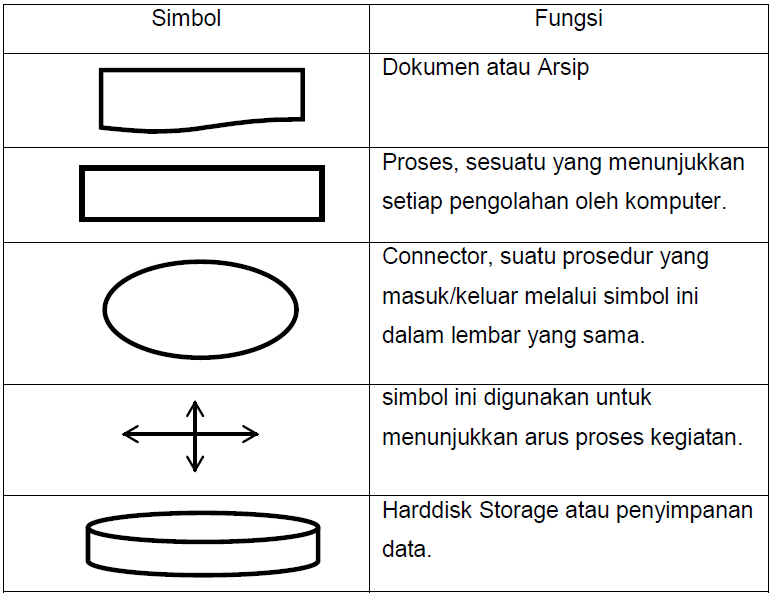
\includegraphics[width=10cm]{gambar/simbolflowchart.png} 

Gambar 1. Simbol Flowchart
\end{center}

\subsection{Diagram Konteks}
Diagram konteks adalah sebuah diagram sederhana yang menggambarkan hubungan antara entiti luar, masukan dan keluaran dari sistem. Diagram konteks direpresentasikan dengan lingkaran tunggal yang mewakili keseluruhan sistem. Berikut adalah contoh diagram konteks:

\begin{center}
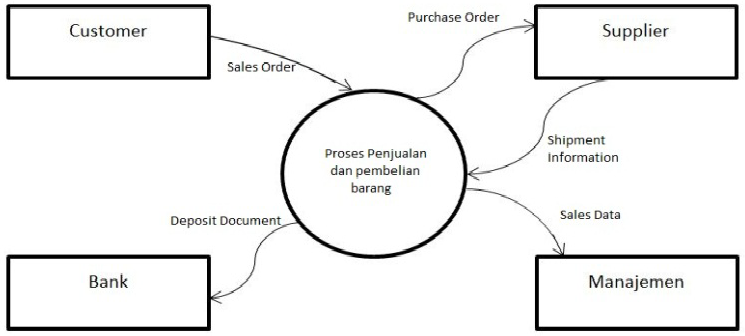
\includegraphics[width=10cm]{gambar/diagramkonteks.png} 

Gambar 2. Diagram Konteks
\end{center}

\subsection{Data Flow Diagram (DFD)}
DFD (Data Flow Diagram) adalah suatu model logika data atau proses yang dibuat untuk menggambarkan darimana asal data dan kemana tujuan data yang keluar dari sistem, dimana data disimpan, proses apa yang menghasilkan data tersebut dan interaksi antara data yang tersimpan dan proses yang dikenakan pada data tersebut. DFD menggambarkan penyimpanan data dan proses yang mentransformasikan data. DFD menunjukkan hubungan antara data pada sistem dan proses pada sistem. Ada 2 teknik dasar DFD yang umum dipakai yaitu Gane and Sarson dan Yourdon and De Marco. Berikut adalah simbol DFD yang dipakai untuk menggambarkan data:
\begin{center}
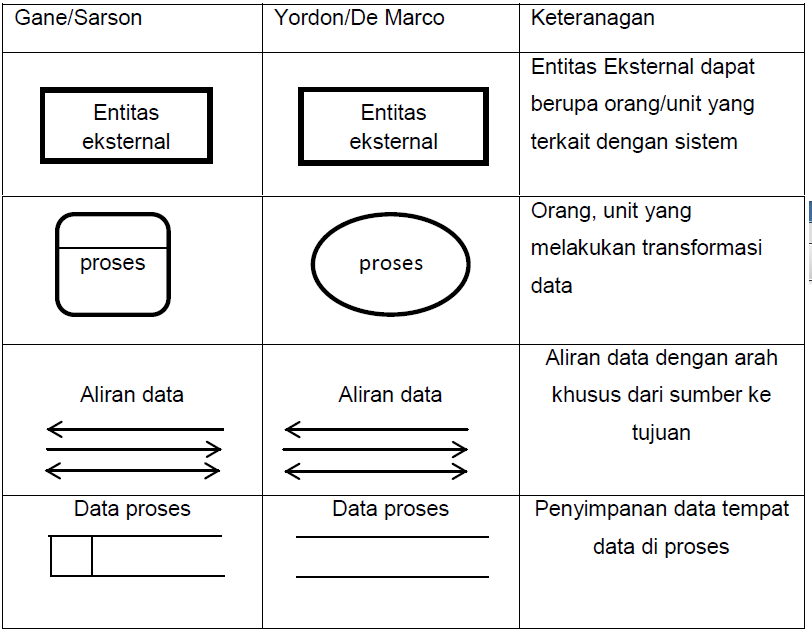
\includegraphics[width=10cm]{gambar/simbolDFD.png} 

Gambar 3. Simbol DFD
\end{center}

\subsection{Konsep Basis Data}
Menurut(Fathansyah (2012), Basis Data, Informatika Bandung, Bandung) Basis data (Database) sediri dapat didefinisikan dalam sejumlah sudut pandang seperti:
\begin{enumerate}
\item Himpunan kelompok data (arsip) yang saling berhubungan yang diorganisasikan sedemikian rupa agar kelak dapat dimanfaatkan kembali dengan cepat dan mudah.
\item Kumpulan data yang saling berhubungan yang disimpan secara bersama sedemikian rupa dan tanpa pengulangan (redundansi) yang tidak perlu, untuk memenuhi berbagai kebutuhan.
\item Kumpulan file/table/arsip yang saling berhubungan yang disimpan dalam media penyimpanan elektronik.
\end{enumerate}

Database merupakan salah satu komponen yang penting di sistem informasi, karena berfungsi sebagai basis penyedia informasi bagi para pemakainya. Penerapan database dalam sistem informasi disebut dengan database sistem. Sistem basis data ( database system ) ini adalah suatu sistem informasi yang mengintegrasikan kumpulan dari data yang saling berhubungan satu dengan lainnya dan membuatnya tersedia untuk beberapa aplikasi yang bermacam-macam di dalam suatu organisasi.

\subsection{Normalisasi}
Normalisasi adalah suatu teknik untuk mengorganisasi data ke dalam tabel-tabel untuk memenuhi kebutuhan pemakai di dalam suatu organisasi.

Perancangan normalisasi bertujuan agar tidak terjadi redudansi data. Jika kondisi tabel tidak terdapat redudansi maka kondisi tabel normal.

Bentuk unnormal merupakan kumpulan data yang akan direkam, tidak ada keharusan mengikuti suatu format tertentu dapat saja data tidak lengkap atau terduplikasi, data dikumpulkan apa adanya.
Bentuk normal pertama adalah tabel yang tidak mengandung pengulangan data. Bentuk normal tahap pertama terpenuhi jika sebuah tabel tidak memiliki atribut bernilai banyak atau lebih dari satu atribut.
Bentuk normal tahap kedua terpenuhi jika pada sebuah tabel, semua atribut yang tidak termasuk dalam key primer memiliki ketergantungan fungsional pada key primer secara utuh. Maka atribut tersebut akan dijadikan satu.

Bentuk normal ketiga memiliki ketentuan harus telah berbentuk normal kedua (2NF) dan relasi tidak boleh memuat kebergantungan fungsional di antara atribut-atribut bukan utama. Bentuk normal ketiga menghilangkan kebergantungan transitif, awalnya bentuk normal ketiga dipikir sebagai bentuk normal puncak atau paling akhir.

\subsection{Tabel Relasi}
Relasi tabel disebut juga relasi antar tabel yaitu menggambarkan hubungan antara file-file yang ada pada suatu pengolahan data. Proses pengelompokan data elemen menjadi tabel-tabel yang menunjukkan entity dan relasinya yang berfungsi untuk menentukan kunci yang mengakses data item atau merupakan database relation sedemikian rupa sehingga database tersebut menjadi dimodifikasi.

\subsection{Entity Relationship Diagram(ERD)}
ERD adalah bentuk bagan yang menggunakan relasi entitas suatu informasi. Entitas relasi diagram dibuat dengan menggunakan persepsi yang terdiri dari sekumpulan objek dasar yaitu entitas dan hubungan antar entitas. Derajat keterhubungan antar entitas pada suatu relasi tersebut dengan kardinalitas. Terdapat tiga jenis kardinalitas diantaranya:
\begin{enumerate}
\item 1-1 : Menunjukan hubungan satu ke satu
\item 1-N : Menunjukan hubungan satu ke banyak
\item N-N : Menunjukan hubungan banyak ke banyak
\end{enumerate}

\subsection{Sistem Absensi}
Menurut Kamus Besar Bahasa Indonesia (Departemen Pendidikan Nasional, "Kamus Besar Bahasa Indonesia Pusat Bahasa Edisi Keempat", Jakarta :PT. Gramedia Pustaka Utama, 2008.), absen adalah tidak masuknya seorang siswa/pegawai pada saat hari masuk/kerja karen sakit, izin, alpa, atau cuti. Sedangkan absensi adalah daftar kehadiran pegawai/siswa, yang berisi jam datang, jam pulang, serta alasan/keterangan kehadiran pegawai.

\subsection{Short Message Service (SMS) Gateway}
Short Message Sevice (SMS) adalah salah satu fasilitas dari teknologi GSM yang memungkinkan mengirim dan menerima pesan pesan singkat berupa teks dari Mobile Station (MS). Menurut Wahidin (Aplikasi SMS dengan PHP untuk Orang Awam, Maxikom. Palembang. (2010)) SMS adalah layanan yang dipakai dalam sistem pengiriman dan penerimaan teks antar telepon selular.

Layanan SMS merupakan sebuah layanan yang bersifat nonreal time dimana sebuah short message dapat di-submit ke suatu tujan, tidak peduli apakah tujuan tersebut aktif atau tidak. Bila dideteksi bahwa tujuan tidak aktif, maka sistem akan menunda pengiriman ke tujuan hingga tujuan aktif kembali. Pada dasarnya sistem SMS akan menjamin delivery dari suatu short message hingga sampai ketujuan. (Edison, Daud Tarigan (2012), Membangun SMS Gateway Berbasis Web Dengan Codeigniter, Lokomedi, Yogyakarta.)

Cara kerja SMS dimulai dari SMS dikirim dari pengirim ke penerima melewati SMSC dengan prinsip Store and Forward, dimana pesan yang dikirim ke SMSC akan disimpan terlebih dahulu hingga masa validitas tertentu terpenuhi jika ponsel nomor yang dituju dalam keadaan mati ataupun diluar jangkauan operator, setelah ponsel nomor yang dituju sudah aktif atau berada dalam jangkauan operator maka pesan akan diteruskan oleh SMSC kepada penerima. Apabila pesan yang tersimpan di SMSC sudah melewati masa validitas yang ditentukan, pesan tersebut akan dihapus dan tidak akan diteruskan kepada nomor yang dituju. (Edison, Daud Tarigan (2012), Membangun SMS Gateway Berbasis Web Dengan Codeigniter, Lokomedi, Yogyakarta.)

Berdasarkan pengertian mengenai SMS dan gateway, maka SMS gateway dapat diartikan sebagai pintu gerbang atau jalur bagi penyebaran informasi dengan menggunakan pesan singkat melalui telephone genggam. Dengan adanya SMS gateway, kita dapat menyebarkan pesan yang akan dikirim itu sekaligus secara otomatis dan cepat ke banyak nomor. (Edison, Daud Tarigan (2012), Membangun SMS Gateway Berbasis Web Dengan Codeigniter, Lokomedi, Yogyakarta.)

\subsection{Perangkat Lunak}
\textbf{Visual Basic 6.0}
Visual Basic adalah bahasa pemograman komputer. Bahasa pemograman adalah perintah-perintah atau instruksi yang dimengerti oleh komputer untuk melakukan tugas-tugas tertentu. Microsoft Visual Basic 6.0 merupakan aplikasi program yang dibuat oleh Microsoft. Visual Basic 6.0 berjalan dalam sistem operasi Windows dan tergabung dalam suite aplikasi Microsoft Visual Studio 6.0. (Bunafit Nugroho, 2014, Membuat Aplikasi Kelinik dengan Visual Basic 6, PT Elex Media Komputindo, Jakarta).

\textbf{Microsoft Access}
Menurut Hear Talib (Panduan Lengkap Microsoft Access 2010, PT Elex Media Komputindo, 2011) Access adalah bagian dari Microsoft Office, merupakan tool untuk mengelola dan mengolah database. Kemampuan yang disediakan Access untuk membantu program aplikasi adalah untuk memudahkan pemakai database lain(database user) untuk memasukkan data, menjalankan prosedur pengolahan data, dan menampilkan informasi. Hal ini berkaitan dengan otomatisasi pekerjaan dan untuk memudahkan pemakaian aplikasi yang awam(casual user).

\textbf{Crystal Reports}
Crystal Reports merupakan salah satu paket program yang digunakan untuk membuat, menganalisa, dan menterjemahkan informasi yang terkandung dalam database ke dalam berbagai jenis laporan.
Crystal Reports dirancang untuk membuat laporan yang dapat digunakan dengan berbagai bahasa pemrograman berbasis Windows, seperti Visual Basic, Visual C/C++, Visual Interdev, dan Borland Delphi.

\section{System Development Life Cycle (SDLC)}
System Development Life Cycle (SDLC) dapat dianggap sebagai kerangka kerja formal tertua metodologi untuk membangun system informasi. Ide utama dari SDLC adalah “untuk mengajar pengembangan system informasi dalam cara yang terstruktur dan metodis, yang mengharuskan tahap Life Cycle dari mulai ide awal sampai pada pengiriman tahap final system, untuk dilaksanakan secara beraturan”. Salah satu tipe SDLC yang paling awal dan paling banyak digunakan adalah metode Waterfall. (McLeod, Sistem Informasi Manajemen, Salemba. 2009).





%-------------------------------------------------------------------------------
\chapter{METODOLOGI PENELITIAN}

\section{Analisis Kebutuhan Sistem}
Komputer terdiri dari perangkat keras dan perangkat lunak yang saling berinteraksi. Perangkat lunak memberikan instruksi-instruksi kepada perangkat keras untuk melakukan suatu tugas tertentu, sehingga dapat menjalankan suatu sistem di dalamnya. Perangkat keras yang dibutuhkan untuk membangun aplikasi sistem absensi berbasis SMS gateway ini adalah sebagai berikut:
\begin{enumerate}
\item Processor minimal 2.0 GHz.
\item RAM 1GB
\item VGA 64 MB
\item Harddisk minimal 40 GB
\item Modem Speedy
\item Print Canon
\end{enumerate}

Perangkat lunak digunakan dalam sebuah sistem merupakan perintah perintah yang diberikan kepada perangkat keras agar bisa saling berinteraksi diantara keduanya. Perangkat lunak yang dibutuhkan untuk membangun aplikasi sistem absensi berbasis SMS gateway ini adalah sebagai berikut:
\begin{enumerate}
\item Sistem Operasi Windows 7
\item Visual basic 6
\item 3. Crystal Report 8.5
\item Ms. Access
\item Adobe Photoshop
\item Notepad
\end{enumerate}

\section{Metode Pengumpulan Data}
Untuk memperoleh data sebagai bahan penulisan tugas akhir dan pembahasan masalah, penulis menggunakan metode sebagai berikut:
\subsection{Observation atau Pengamatan}
Observation adalah pengumpulan data dengan cara pengamatan secara langsung terhadap obyek penelitian. Observation ini merupakan salah satu teknik pengumpulan data yang cukup efektif dan efisien untuk mempelajari system yang ada. Metode ini dilakukan dengan cara mengamati langsung suatu kegiatan yang sedang dilakukan, dalam hal ini penulis mengadakan pengamatan pada system dan prosedur yang berjalan pada SMKN 5 JEMBER.
\subsection{lnterview atau Wawancara}
Metode ini dilakukan dengan cara melakukan tanya jawab secara langsung dengan berbagai pihak yang terkait dalam proses pembuatan dan perancangan aplikasi surat, yang dapat memberikan data-data yang diperlukan yang berguna dalam penulisan laporan akhir studi ini.
\subsection{Tinjauan Pustaka}
Tinjauan pustaka ini merupakan metode yang dilakukan dengan cara rnembaca, mencatat, mengutip dan meresume buku-buku yang berkaitan dengan aplikasi sehingga mendukung pengumpulan data yang berhubungan dengan penelitian. Dalam tinjauan pustaka ini penulis mencari sumber pustaka baik dari buku pegangan dan peraturan yang tertulis ataupun pedoman kerja diperusahaan serta sumber-sumber lain yang mendukung.

\section{Identifikasi Masalah}
Identifikasi masalah dilakukan dengan cara mempelajari masalah-masalah yang timbul dalam Tata system informasi. Masalah yang timbul sebelum system ini diciptakan ialah: 
\begin{enumerate}
\item Proses penginputan data pasien dan catatan medis pasien memakan waktu yang lama, dikarenakan proses penginputan masih bersifat manual. 
\item Proses pencarian data dan pemrosesan data yang dibutuhkan juga akan memakan waktu yang lama dikarenakan system informasi pada klinik yang awalnya masih bersifat manual.
\end{enumerate}

\section{Perancangan Sistem}
Perancangan Sistem merupakan tahapan dalam memproses data yang sudah dikumpulkan untuk dibangun sebuah aplikasi. Berikut perancangan sistemnya:

\begin{center}
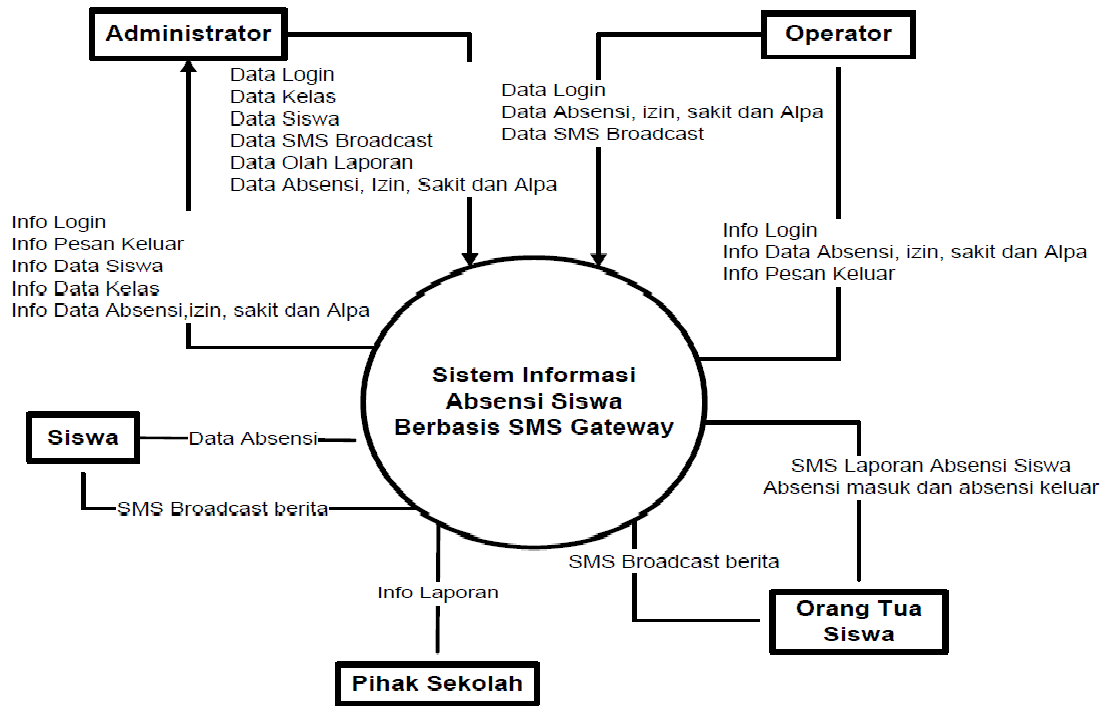
\includegraphics[width=10cm]{gambar/perancangansistem.png} 

Gambar 5. Perancangan Sistem
\end{center}


\section{Jadwal Kegiatan}
Rincian rencana jadwal penelitian dicantumkan dalam tabel berikut.

3.1 Tabel Jadwal Kegiatan Penelitian

\begin{center}
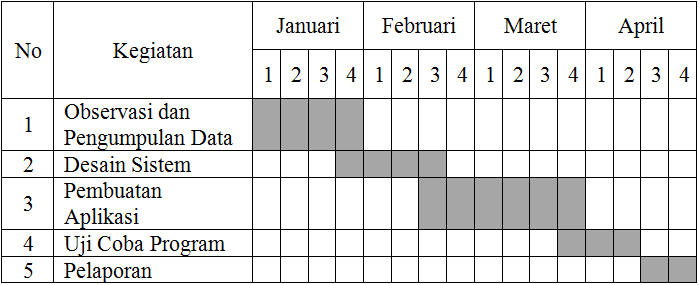
\includegraphics[width=13cm]{gambar/jadwal.png} 
\end{center}




%-----------------------------------------------------------------
%Disini akhir masukan Bab
%-----------------------------------------------------------------

%-----------------------------------------------------------------
%Disini awal masukan untuk Daftar Pustaka
%-----------------------------------------------------------------
%%\nocite{Abel2010,Guerbas201350}
%%\bibliography{research-plan}
%%\bibliographystyle{plainnat}
\begin{thebibliography}{9}

\bibitem[satu(2013)]{satu01}
Bambang Hartono. 2013. Sistem informasi Manajemen Berbasis Komputer. Jakarta: PT Rineka Cipta.

\bibitem[dua(2015)]{dua02}
Departemen Pendidikan Nasional. 2008. Kamus Besar Bahasa Indonesia Pusat Bahasa Edisi Keempat. Jakarta: PT. Gramedia Pustaka Utama.

\bibitem[tiga(2015)]{tiga03}
Edison, Daud Tarigan. 2012. Membangun SMS Gateway Berbasis Web Dengan Codeigniter.Yogyakarta: Lokomedi.

\bibitem[empat(2015)]{tiga04}
Saputro, H., Sugiri. 2008. Pengelolaan Database Mysql Dengan Phpmyadmin. Yogyakarta: Graha Ilmu.

\end{thebibliography}
\addcontentsline{toc}{chapter}{DAFTAR PUSTAKA}
%-----------------------------------------------------------------
%Disini akhir masukan Daftar Pustaka
%-----------------------------------------------------------------

\end{document}